Web Services bieten eine auf Standards basierende Technologie, um SOAs zu realisieren. Mittlerweile setzen viele gro�e Softwarekonzerne auf Web Services und haben ihre Produktstrategien entsprechend ausgerichtet.
Als Web-Service bezeichnet man im Allgemeinen eine Softwarekomponente, die
ihre Funktionalit�t �ber Standardinternetprotokolle zur Verf�gung stellt.
W3C definiert die Web Services folgenderma�en: 
\begin{Def}
A software application identified by a URI, whose interfaces and bindings are capable of being
defined, described, and discovered as XML artifacts. A Web service supports direct interactions
with other software agents using XML-based messages exchanged via Internet-based protocols.(W3C)
\end{Def}


W�hrend die erste Definition die konkreten Interaktionsprotokollen und die Beschreibungssprache f�r die Schnittstellen noch offen l�sst, werden in der n�chste Definition die  wichtigen Standards genannt. 
\begin{Def}
A Web service is a software system designed to support interoperable machine-to-machine
interaction over a network. It has an interface described in a machine-processable format
(specifically WSDL). Other systems interact with the Web service in a manner prescribed by its
description using SOAP messages, typically conveyed using HTTP with an XML serialization in
conjunction with other Web-related standards (W3C 2004a).
\end{Def}

Gem�� der beiden Definitionen sind die Beschreibung von Schnittstellen und
der Nachrichtenaustausch wesentliche Aufgaben. SOAP, WSDL und UDDI sind die daf�r vorgesehen Standards und bilden den Kern der Web Services.
\begin{itemize}
	\item SOAP ein standardisiertes, XML-basiertes
Protokoll zum Verpacken von Nachrichten, die zwischen Applikationen ausgetauscht
werden. SOAP setzt auf Transportschicht auf und ist dadurch von dem verwendeten Transportprotokoll unabh�ngig. Am H�ufigsten wird der HTTP-Protokoll eingesetzt.
\item UDDI (Universal Description, Discovery and Integration) dient zur Lokalisierung und Ver�ffentlichung
von Web-Services im Internet. UDDI bietet Standardfunktionen zum Klassifizieren,
Katalogisieren und Verwalten von Metadaten �ber Web-
Services.
\item WSDL (Web Services Defnition Language) ist eine funktionale, XML-basierte Beschreibungssprache
f�r die Schnittstellen eines Web Services.(siehe n�chsten Abschnitt)
\end{itemize}
In der Abbildung \ref{fig:wsTechnologieStack} sind die genannten Standards in Web Service-Technologiestack eingeordnet.  

\begin{figure}[htbp]
	\centering
		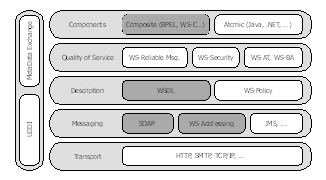
\includegraphics[width=0.75\textwidth]{bilder/wsTechnologieStack.png}
		\caption{Web Service Technologie Stack}
	\label{fig:wsTechnologieStack}
\end{figure}

Der Zusammenhang dieser Standards und die grundlegende Funktionsweise ist in der Abbildung \ref{fig:WSFunktionsweise} dargestellt. Web Service-Architektur unterscheidet die Rollen Service-Anbieter, Service-Nutzer
und Service-Verzeichnis. Ein Service-Anbieter registriert Informationen �ber von ihm bereitgestellte Dienste bei einem
Dienst-Verzeichnis. Ein Dienst-Nutzer nutzt das Dienst-Verzeichnis zum Auffinden
existierender Dienst-Implementierungen und startet die Interaktion mit
der gew�hlten Dienst-Komponente.
\begin{figure}[htbp]
	\centering
		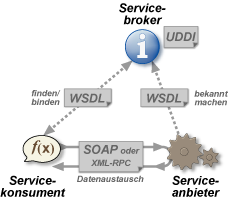
\includegraphics[width=0.65\textwidth]{bilder/Webservice.png}
		\caption{Rollen und Standards in einer Web Service-Architektur}
	\label{fig:WSFunktionsweise}
\end{figure}

Web Services stellen eine L�sung f�r die Integration von verschiedenen, autonomen Systemen dar. Die immer wiederkehrenden Funktionen im Unternehmen werden nur einmal implementiert und anderen Programmen als Services zur Verf�gung gestellt. Dadurch k�nnen Redundanzen vermieden und
Kosten in der Entwicklung gesenkt werden.
